%% abtex2-modelo-projeto-pesquisa.tex, v<VERSION> laurocesar
%% Copyright 2012-2015 by abnTeX2 group at http://www.abntex.net.br/ 
%%
%% This work may be distributed and/or modified under the
%% conditions of the LaTeX Project Public License, either version 1.3
%% of this license or (at your option) any later version.
%% The latest version of this license is in
%%   http://www.latex-project.org/lppl.txt
%% and version 1.3 or later is part of all distributions of LaTeX
%% version 2005/12/01 or later.
%%
%% This work has the LPPL maintenance status `maintained'.
%% 
%% The Current Maintainer of this work is the abnTeX2 team, led
%% by Lauro César Araujo. Further information are available on 
%% http://www.abntex.net.br/
%%
%% This work consists of the files abntex2-modelo-projeto-pesquisa.tex
%% and abntex2-modelo-references.bib
%%

% ------------------------------------------------------------------------
% ------------------------------------------------------------------------
% abnTeX2: Modelo de Projeto de pesquisa em conformidade com 
% ABNT NBR 15287:2011 Informação e documentação - Projeto de pesquisa -
% Apresentação 
% ------------------------------------------------------------------------ 
% ------------------------------------------------------------------------

\documentclass[
	% -- opções da classe memoir --
	12pt,				% tamanho da fonte
	openright,			% capítulos começam em pág ímpar (insere página vazia caso preciso)
	oneside,			% para impressão em recto e verso. Oposto a oneside
	a4paper,			% tamanho do papel. 
	% -- opções da classe abntex2 --
	%chapter=TITLE,		% títulos de capítulos convertidos em letras maiúsculas
	%section=TITLE,		% títulos de seções convertidos em letras maiúsculas
	%subsection=TITLE,	% títulos de subseções convertidos em letras maiúsculas
	%subsubsection=TITLE,% títulos de subsubseções convertidos em letras maiúsculas
	% -- opções do pacote babel --
	english,			% idioma adicional para hifenização
	brazil,				% o último idioma é o principal do documento
	]{abntex2}


% ---
% PACOTES
% ---

% ---
% Pacotes fundamentais 
% ---
\usepackage{lmodern}			% Usa a fonte Latin Modern
\usepackage[T1]{fontenc}		% Selecao de codigos de fonte.
\usepackage[utf8]{inputenc}		% Codificacao do documento (conversão automática dos acentos)
\usepackage{indentfirst}		% Indenta o primeiro parágrafo de cada seção.
\usepackage{color}				% Controle das cores
\usepackage{graphicx}			% Inclusão de gráficos
\usepackage{microtype} 			% para melhorias de justificação
\usepackage{amsmath,amssymb,amstext}

% ---
% Pacotes e definições adcionais, para adequações especificas
\usepackage{tikz}				
\usepackage{pdflscape}			% para ambiente landscape
\usepackage{pgfgantt}			% cronograma estilo gráfico de gantt

\definecolor{done}{RGB}{120, 180, 120}
\definecolor{do}{RGB}{180, 120, 120}
% ---

% ---
% Pacotes adicionais, usados apenas no âmbito do Modelo Canônico do abnteX2
% ---
\usepackage{lipsum}				% para geração de dummy text
% ---

% ---
% Pacotes de citações
% ---
\usepackage[brazilian,hyperpageref]{backref}% Paginas com as citações
\usepackage[alf]{abntex2cite}				% Citações padrão ABNT

% --- 
% CONFIGURAÇÕES DE PACOTES
% --- 

% ---
% Configurações do pacote backref
% Usado sem a opção hyperpageref de backref
\renewcommand{\backrefpagesname}{Citado na(s) página(s):~}
% Texto padrão antes do número das páginas
\renewcommand{\backref}{}
% Define os textos da citação
\renewcommand*{\backrefalt}[4]{
	\ifcase #1 %
		Nenhuma citação no texto.%
	\or
		Citado na página #2.%
	\else
		Citado #1 vezes nas páginas #2.%
	\fi}%
% ---

% ---
% Informações de dados para CAPA e FOLHA DE ROSTO
% ---
\titulo{Extensões e Aplicações Modelo de Regressão
Conway-Maxwell-Poisson para Modelagem de Dados de Contagem}
\vspace{2cm}}
\autor{Eduardo Elias Ribeiro Junior}
\local{Curitiba}
\data{2015}
\instituicao{}
\tipotrabalho{Projeto de Pesquisa}
% O preambulo deve conter o tipo do trabalho, o objetivo, 
% o nome da instituição e a área de concentração 
\preambulo{Projeto de Pesquisa apresentado à disciplina Laboratório A 
do Curso de Graduação em Estatística da Universidade Federal do Paraná, 
como requisito para elaboração do Trabalho de Conclusão de Curso}
% ---

% ---
% Configurações de aparência do PDF final

% alterando o aspecto da cor azul
\definecolor{blue}{RGB}{41,5,195}

% informações do PDF
\makeatletter
\hypersetup{
     	%pagebackref=true,
		pdftitle={\@title}, 
		pdfauthor={\@author},
   	 	pdfsubject={\imprimirpreambulo},
	    pdfcreator={LaTeX with abnTeX2},
		pdfkeywords={abnt}{latex}{abntex}{abntex2}{projeto de pesquisa}, 
		colorlinks=true,	% false: boxed links; true: colored links
  	  	linkcolor=blue,     % color of internal links
    		citecolor=blue, % color of links to bibliography
    		filecolor=magenta, % color of file links
		urlcolor=blue,
		bookmarksdepth=4
}
\addto\captionsbrazil{
	\renewcommand{\bibname}{\uppercase{REFER\^ENCIAS}}
}
\makeatother
% --- 

% --- 
% Espaçamentos entre linhas e parágrafos 
% --- 

% O tamanho do parágrafo é dado por:
\setlength{\parindent}{1.3cm}

% Controle do espaçamento entre um parágrafo e outro:
\setlength{\parskip}{0.2cm}  % tente também \onelineskip

% ---
% compila o indice
% ---
\makeindex
% ---

% ----
% Início do documento
% ----
\begin{document}

% Seleciona o idioma do documento (conforme pacotes do babel)
%\selectlanguage{english}
\selectlanguage{brazil}

% Retira espaço extra obsoleto entre as frases.
%\frenchspacing 

% ----------------------------------------------------------
% ELEMENTOS PRÉ-TEXTUAIS
% ----------------------------------------------------------
% \pretextual

% ---
% Capa
% ---
\tikz[remember picture,overlay] \node[opacity=0.9,inner sep=0pt] at 
	(current page.center){
		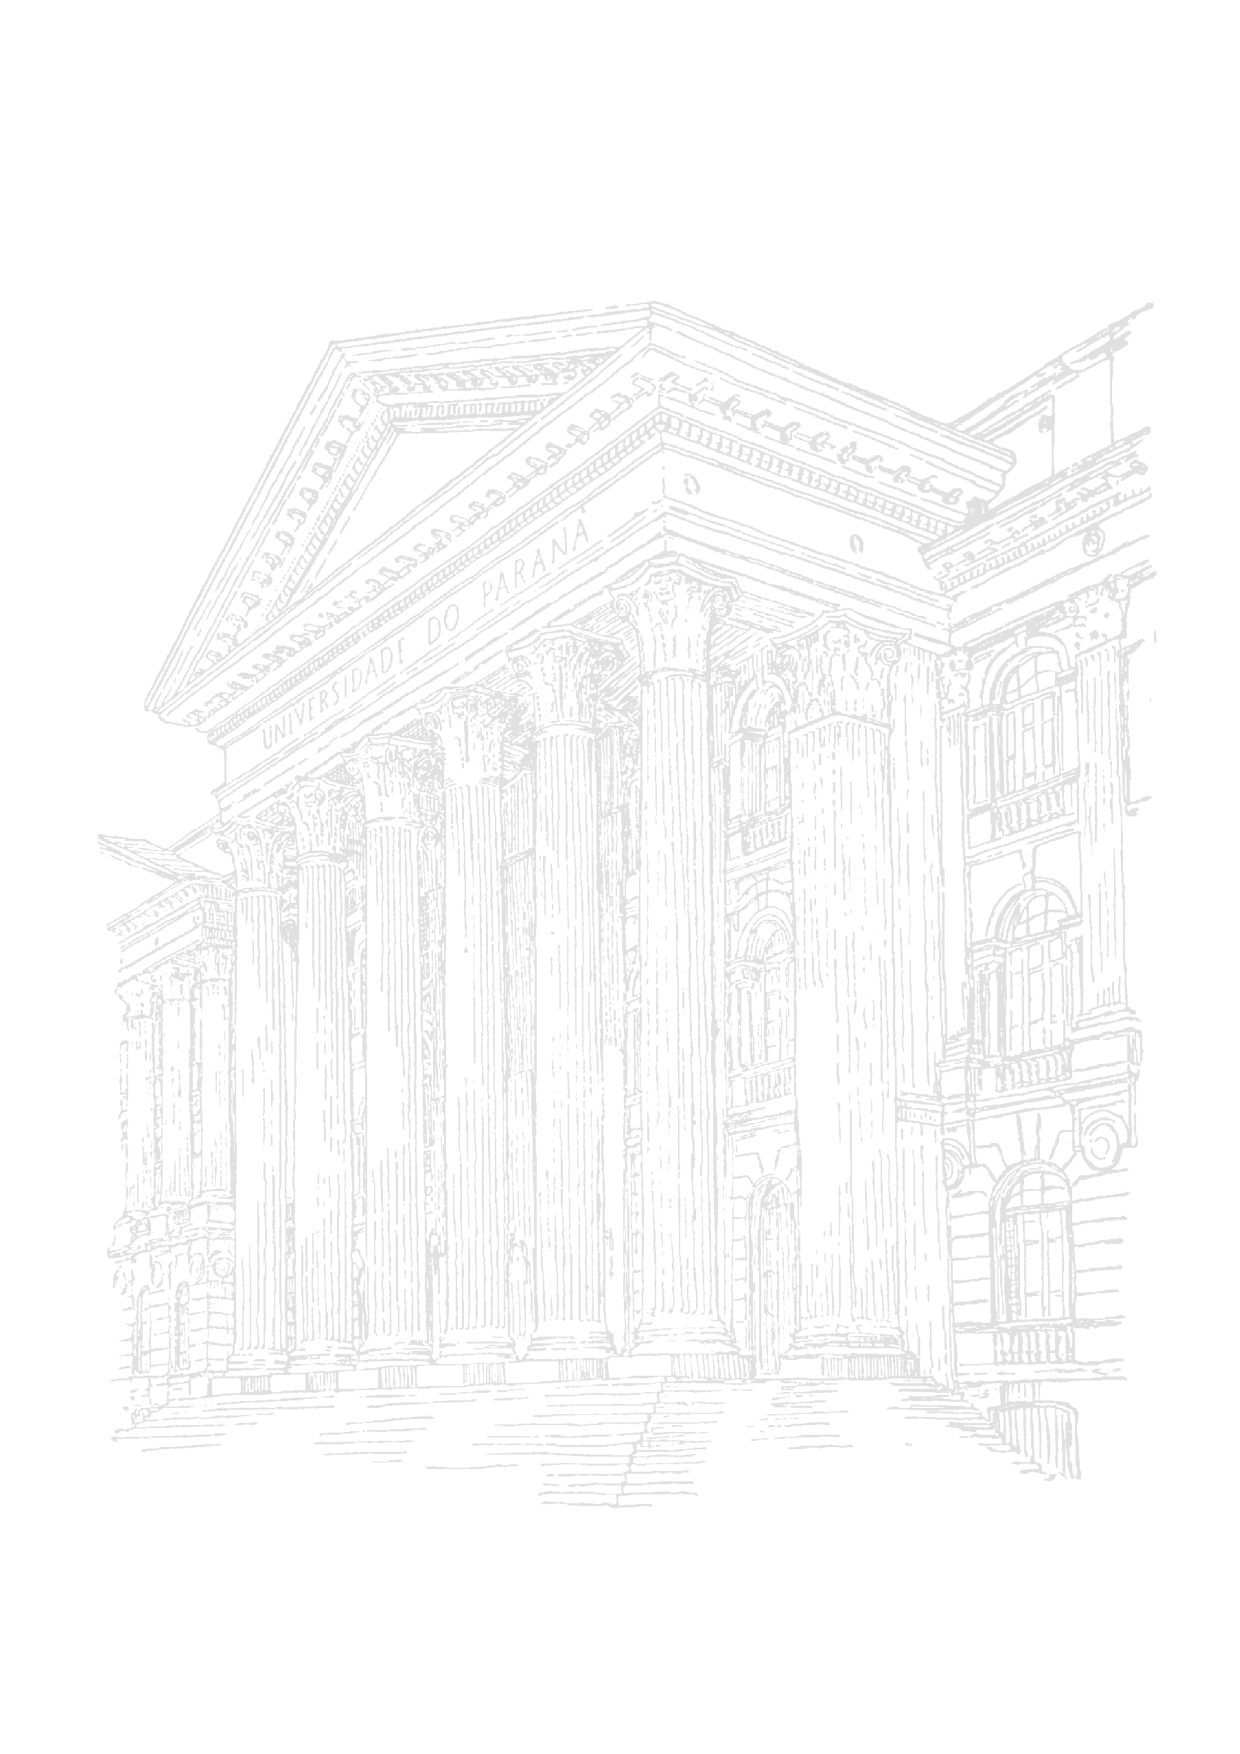
\includegraphics[width=\paperwidth,
						height=\paperheight]{figures/ufpr_bg}};

\begin{center}
{\Large \textsf{Universidade Federal do Paraná}} \\
\end{center}
\imprimircapa

% ---

% ---
% Folha de rosto
% ---
\imprimirfolhaderosto
% ---

% ---
% inserir o sumario
% ---
\pdfbookmark[0]{\contentsname}{toc}
\tableofcontents*
\cleardoublepage
% ---


% ----------------------------------------------------------
% ELEMENTOS TEXTUAIS
% ----------------------------------------------------------
\textual

% ----------------------------------------------------------
% Introdução
% ----------------------------------------------------------
\chapter{Introdução}

Discutir a relevância e aplicação de modelos estatísticos de regressão
no âmbito científico: compreender e medir a relação entre uma varíavel
dependente com variáveis independentes e fazer previsão.

Descrever a estrutura genérica de um modelo de regressão: variável
resposta, variáveis preditoras, distribuição de probabilidades,
especificação do preditor, função de ligação.

Tipo de modelos de regressão. Modelos lineares quando a variável é
normal. GLM é uma extensão para respostas não Gaussinas.  Citar a
introdução dos modelos lineares generalizados.  Poisson é o membro da
familia para dados de contagem.

O processo de Poisson. As características de uma v.a. Poisson. A
restrição da suposição de equidispersão. Mecanísmos geradores de
contagens.

Abordar modelos de regressão para variáveis de contagem, descrever as
características, e com isso a imitação do modelo de regressão Poisson.

Apresentar o modelo COM-Poisson. Enfatizar sua flexibilidade,
principalmente para casos de subdispersão.

Abordar modelos lineares mistos com situações exemplos, e discutir a
aplicação de modelos mistos para acomodar sobredispersão. Comentar que,
até onde temos conhecimento, não existem aplicações/implementações do
COM-Poisson com efeito aleatório.

Da mesma forma, modelos com inflação de zeros e contagem COM-Poisson não
foram encontrados.

Comentar dos problemas de cunho númerico relacionado a COM-Poisson que
merecem cuidados na implementação ao são desafiadores. A constante de
integração que exige uma soma infinita, o expoentes altos. Os métodos de
integração para modelos de efeito aleatório.

Ressaltar a relevância do estudo para a comunidade estatística,
principalmente como contribuição para a literatura estatística
brasileira.

% ----------------------------------------------------------
% Objetivos
% ----------------------------------------------------------
\chapter{Objetivos}
\section{Objetivos Gerais}

Apresentar o modelo de regressão COM-Poisson, alternativa 
paramétrica não comumente utilizada pela comunidade de 
Estatística aplicada, trazendo discussões sobre aspectos 
inferenciais deste modelo. Estender as aplicações do modelo
COM-Poisson para situações específicas (efeitos aleatórios 
e inflação de zeros).

\section{Objetivos Específicos}

\begin{itemize}
\item Apresentar e discutir aspectos da distribuição COM-Poisson para
  modelos de regressão para dados de contagem;
	
\item Avaliar as propriedades de soluções númericas para 1) cálculo da
  densidade de probabilidade do modelo e 2) para estimação de modelos de
  regressão de efeito fixo;
	
\item Propor e implementar uma extensão do modelo de regressão
  COM-Poisson para acomodar efeitos aleatórios;
	
\item Propor e implementar uma extensão do modelo de regressão
  COM-Poisson para acomodar contagens com excesso de zeros.
	
\item Fazer a aplicação do modelo COM-Poisson e das extensões
  desenvolvidas à dados reais ou simulados. Fazer comparações com os
  modelos disponíveis para as situações estudadas: Poisson,
  Quasi-Poisson, Binomial Negativo, Poisson de efeito aleatório.
\end{itemize}

% ----------------------------------------------------------
% Materiais e Métodos
% ----------------------------------------------------------
\chapter{Materiais e Métodos}
\section{Materiais}

\subsection{Dados para análise}

Descrever os conjuntos de dados reais a serem utilizados no 
trabalho de conclusão de curso. Inicialmente temos os 
conjuntos \texttt{defoliation}, do pacote \texttt{legTools}
também analisado via modelo de contagem Gama 
\cite{Zeviani2014}, e o conjunto \texttt{aviurba}, do pacote
\texttt{ade4} de análise de dados ecológicos, onde se pode 
aplicar um modelo de efeitos fixos e aleatórios.

Descrever os procedimentos de simulação de dados para 
avaliação da acurácia dos métodos de estimação e comparação 
de abordagens distintas.

\subsection{Recursos Computacionais}

Para análise e elaboração do trabalho será utilizado o
\textit{software R}, na versão 3.2 \cite{Rcore2015}. 
Atualmente há três bibliotecas desenvolvidas em R dedicadas
à distribuição COM-Poisson. São eles \texttt{COMPoissonReg}
\cite{COMPoissonReg}, este conjunto de funções foi 
desenvolvido com base nas análises apresentadas no artigo
\textit{A flexible regression model for count data} 
\cite{Sellers2010}; \texttt{compoisson} as funções desta 
biblioteca se dedicam apenas ao modelo probabilístico; e
\texttt{CompGLM} esta é mais recente biblioteca de funções 
com ênfase no modelo COM-Poisson, escrita em \texttt{C++}
permite a estimação de modelos de regressão além de funções 
probabilísticas.

Outros recursos e bibliotecas, principalmente para 
otimização de funções e elaboração de gráficos, serão 
utilizadas.

\section{Métodos}

Descrever o método de máxima verossimilhança para estimação 
dos modelos de regressão e os critérios a serem utilizados 
para comparação de modelos.

% ----------------------------------------------------------
% Cronograma
% ----------------------------------------------------------
\begin{landscape}
\chapter{Cronograma de Atividades}
%\noindent\resizebox{1.6\textwidth}{!}{
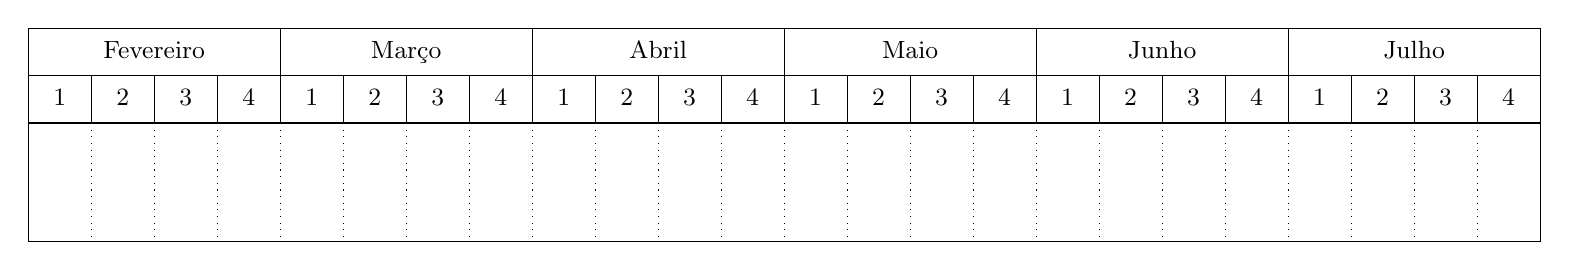
\begin{tikzpicture}[x=.5cm, y=0.5cm]
\begin{ganttchart}[	y unit title=0.6cm, % Size da indicação do tempo
					y unit chart=1.5cm, % Size do altura das colunas
					x unit=8mm,
					vgrid, % grid cinza vertical
					hgrid, % grid cinza horizontal
					title height=1, % Size dos dias
					 % cor das barras a fazer
					bar/.style={draw,fill=done},
					% cor das barras incompletas
					bar incomplete/.append style={fill=do}, 
					bar label node/.append style={align=right},
					bar label font=\bfseries\normalsize\color{black!65},
					%bar height=0.6, % size das barras de tarefas
					bar left shift=.2, bar right shift=-.2,
					bar top shift=.2, bar height=.5,
					%% today=16,
					%% today offset = 0.5,
					%% today label=Hoje,
					%% today label font=\bfseries\color{red},
					%% today rule/.style={draw=red, ultra thick, dotted},
					progress label text ={\pgfmathprintnumber[precision=0, verbatim]{#1}\% realizado},
					newline shortcut=true,]
					{1}{24} % 
\gantttitle{Fevereiro}{4}
\gantttitle{Março}{4} 
\gantttitle{Abril}{4} 
\gantttitle{Maio}{4} 
\gantttitle{Junho}{4} 
\gantttitle{Julho}{4} \\
\gantttitlelist{1,...,4}{1}
\gantttitlelist{1,...,4}{1}
\gantttitlelist{1,...,4}{1}
\gantttitlelist{1,...,4}{1}
\gantttitlelist{1,...,4}{1}
\gantttitlelist{1,...,4}{1} \\
%\ganttgroup[progress=95]{Projeto de Pesquisa}{1}{16} \\
%\ganttbar[progress=100, progress label text=]{Definição \ganttalignnewline do tema}{2}{4} \\
%\ganttbar[progress=100, progress label text= ]{Revisão de \ganttalignnewline literatura}{5}{12} \\
%\ganttbar[progress=100, progress label text= ]{Elaboração do \ganttalignnewline projeto}{10}{15} \\
%\ganttbar[progress=0, progress label text= ]{Apresentação \ganttalignnewline do projeto}{16}{16} \\
%\ganttgroup[progress=8]{Relatório da Pesquisa}{16}{44} \\
%\ganttbar[progress=20]{Revisão de \ganttalignnewline literatura}{17}{35} \\
%\ganttbar[progress=0, progress label text= ]{Análise \ganttalignnewline dos dados}{24}{31} \\
%\ganttbar[progress=0, progress label text= ]{Discussão \ganttalignnewline dos resultados}{32}{35} \\
%\ganttbar[progress=0, progress label text= ]{Produção \ganttalignnewline textual}{35}{40} \\
%\ganttbar[progress=0, progress label text= ]{Elaboração \ganttalignnewline de apresentação}{40}{43} \\
%\ganttbar[progress=0, progress label text= ]{Apresentação \ganttalignnewline do relatório}{44}{44} \\
%% rela\c c\~oes
%\ganttlink{elem1}{elem2}
%\ganttlink{elem2}{elem3}
%\ganttlink{elem3}{elem4}
%\ganttlink{elem6}{elem7}
%\ganttlink{elem6}{elem8}
%\ganttlink{elem6}{elem9}
%\ganttlink{elem7}{elem8}
%\ganttlink{elem8}{elem9}
%\ganttlink{elem9}{elem10}
%\ganttlink{elem10}{elem11}
\end{ganttchart}
\end{tikzpicture}
%}
\\

\end{landscape}

% ---
\phantompart

% ---
% Conclusão
% ---

% ----------------------------------------------------------
% ELEMENTOS PÓS-TEXTUAIS
% ----------------------------------------------------------
\postextual

% ----------------------------------------------------------
% Referências bibliográficas
% ----------------------------------------------------------
\nocite{Paula2013} 
\nocite{RibeiroJr2012} 
\nocite{Shmueli2005} 
\nocite{Conway1962}
\bibliography{compois}


\end{document}
